%% LaTeX-Beamer template for KIT design
%% by Erik Burger, Christian Hammer
%% title picture by Klaus Krogmann
%%
%% version 2.1
%%
%% mostly compatible to KIT corporate design v2.0
%% http://intranet.kit.edu/gestaltungsrichtlinien.php
%%
%% Problems, bugs and comments to
%% burger@kit.edu

\documentclass[18pt]{beamer}

%% SLIDE FORMAT

% use 'beamerthemekit' for standard 4:3 ratio
% for widescreen slides (16:9), use 'beamerthemekitwide'

\usepackage{templates/beamerthemekit}
\usepackage[utf8]{inputenc}
\usepackage[T1]{fontenc}
\usepackage{graphicx}
\usepackage{tikz}
\usepackage{listings}
\usepackage{color}
\usepackage{ifthen}
\usepackage{animate}

% \usepackage{templates/beamerthemekitwide}

%% TITLE PICTURE

% if a custom picture is to be used on the title page, copy it into the 'logos'
% directory, in the line below, replace 'mypicture' with the 
% filename (without extension) and uncomment the following line
% (picture proportions: 63 : 20 for standard, 169 : 40 for wide
% *.eps format if you use latex+dvips+ps2pdf, 
% *.jpg/*.png/*.pdf if you use pdflatex)

\titleimage{sheep}

%% TITLE LOGO

% for a custom logo on the front page, copy your file into the 'logos'
% directory, insert the filename in the line below and uncomment it

%\titlelogo{mylogo}

% (*.eps format if you use latex+dvips+ps2pdf,
% *.jpg/*.png/*.pdf if you use pdflatex)

%% TikZ INTEGRATION

% use these packages for PCM symbols and UML classes
% \usepackage{templates/tikzkit}
% \usepackage{templates/tikzuml}

% the presentation starts here

\title{Abschlusspräsentation der Java-Gruppe}
\subtitle{Neuronale Netze mit Neuroph}
\author{Markus Braun, Daniel Hammann, Dominik Messinger, Dominic Rausch}

\institute{Institut für Programmstrukturen und Datenorganisation (IPD), Lehrstuhl für Programmiersysteme}

% Hier kommt der ganze Quatsch für Listings
\definecolor{javared}{rgb}{0.6,0,0} % for strings
\definecolor{javagreen}{rgb}{0.25,0.5,0.35} % comments 
\definecolor{javapurple}{rgb}{0.5,0,0.35} % keywords
\definecolor{javadocblue}{rgb}{0.25,0.35,0.75} % javadoc
 
\lstset{language=Java,
basicstyle=\ttfamily,
keywordstyle=\color{javapurple}\bfseries,
stringstyle=\color{javared},
commentstyle=\color{javagreen},
morecomment=[s][\color{javadocblue}]{/**}{*/},
numbers=left,
numberstyle=\tiny\color{black},
stepnumber=1,
numbersep=10pt,
tabsize=4,
showspaces=false,
showstringspaces=false}
%\usepackage[citestyle=authoryear,bibstyle=numeric,hyperref,backend=biber]{biblatex}
%\addbibresource{templates/example.bib}
%\bibhang1em

\begin{document}
	\maketitle

	\begin{frame}[c]\frametitle{Neuronale Netze}
		\begin{block}{Einleitung}
		    \begin{itemize}
			    \item Bestehen aus Neuronen (Verarbeitungseinheiten)
		    	\item Gewichtete Eingabeverbindungen werden zusammenfasst (Propagierungsfunktion)
		    	\item Aktivierungsfunktion mit Schwellwert
		    	\item Aus Aktivierung folgt mittels Ausgabefunktion die Ausgabe
		    \end{itemize}		    
		\end{block}	
		\vspace{.5cm}
		\begin{minipage}[c]{0.48\textwidth}
			\begin{center}
			\includegraphics[width=0.5\textwidth]{images/ann.png}
			\end{center}
		\end{minipage}	
		\begin{minipage}[c]{0.48\textwidth}
			\begin{center}
			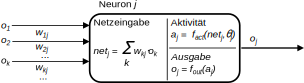
\includegraphics[width=\textwidth]{images/Neuron}
			\end{center}				
		\end{minipage}
		\begin{flushright}
			\tiny{[Quelle: Lehr- und Übungsbuch künstliche Intelligenz; Lämmel, Cleve; 2012]}
		\end{flushright}
	\end{frame}

	%!TEX root = abschlusspraesentation.tex

\begin{frame}[c]\frametitle{NN Auswertung}
\usetikzlibrary{arrows}
\usetikzlibrary{positioning} 
\usetikzlibrary{automata} 

  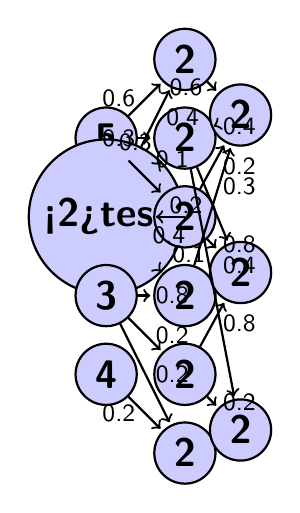
\begin{tikzpicture}[->,shorten >=1pt,auto, node distance=1cm,
    thick,main node/.style={circle,fill=blue!20,draw,font=\sffamily\Large\bfseries}]

    \node[main node] (0) {5};
    \node[main node] (1) [below of=0] {\only<2>{test}};
    \node[main node] (2) [below of=1] {3};
    \node[main node] (3) [below of=2] {4};

    \node[main node] (11) [right of=0] {2};
    \node[main node] (10) [above of=11] {2};
    \node[main node] (12) [right of=1] {2};
    \node[main node] (13) [right of=2] {2};
    \node[main node] (14) [right of=3] {2};
    \node[main node] (15) [below of=14] {2};

    \node[main node] (20) [below right  of=10] {2};
    \node[main node] (21) [below right  of=12] {2};
    \node[main node] (22) [below right  of=14] {2};

    \path[every node/.style={font=\sffamily\small}]
      (0) edge node [left] {0.6} (10)
          edge node[left] {0.3} (11)
          edge node {0.1} (12)
      (1) edge node [right] {0.4} (10)
          edge node {0.3} (11)
          edge node {0.4} (12)
          edge node {0.1} (13)
      (2) edge node [right] {0.8} (13)
          edge node [right] {0.2} (14)
          edge node [right] {0.2} (15)
      (3) edge node [left] {0.2} (15)

      (10)edge node [left] {0.6} (20)
      (11)edge node [right] {0.4} (20)
          edge node {0.3} (21)
          edge node {0.4} (22)
      (12)edge node [right] {0.8} (21)
          edge node [right] {0.2} (20)
      (13)edge node [left] {0.2} (20)
      (14)edge node [right] {0.8} (21)
          edge node [right] {0.2} (22)
      ;
  \end{tikzpicture}    
\end{frame}
	

	\begin{frame}[c]\frametitle{Neuronale Netze}
		\begin{center}
		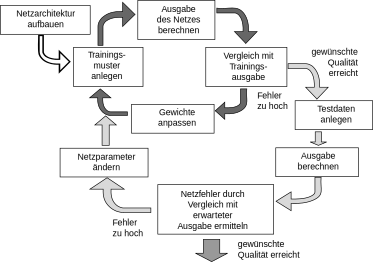
\includegraphics[scale=.8]{images/workflow}
		\end{center}
		\begin{flushright}
		\tiny{[Quelle: Lehr- und Übungsbuch künstliche Intelligenz; Lämmel, Cleve; 2012]}
		\end{flushright}
	\end{frame}		

	\begin{frame}[c]\frametitle{Überblick}
	%TODO: Diese Folie ganz weg?
		\begin{block}{Was bisher geschah}
		    \begin{itemize}
		    	\item Einarbeitung in die Thematik der Neuronale Netze
			    \item Testdaten beschaffen
		    	\item Code Analyse der Simulationsumgebung Neuroph
		    	\item Drei Parallelisierungsversuche
		    	\item Profiling (u.a. eigenes Evaluierungsframework)
		    \end{itemize}		    
		\end{block}
	\end{frame}

	\begin{frame}[c]\frametitle{Code Analyse \& Profiling}
		\begin{block}{Was wir vorgefunden haben}
			\begin{center}
				\includegraphics[scale=0.4]{images/Klassendiagramm.png}
			\end{center}
		\end{block}
	\end{frame}
	
	\begin{frame}[c]\frametitle{Code Analyse: Sequenzdiagramm}
			\begin{center}
			  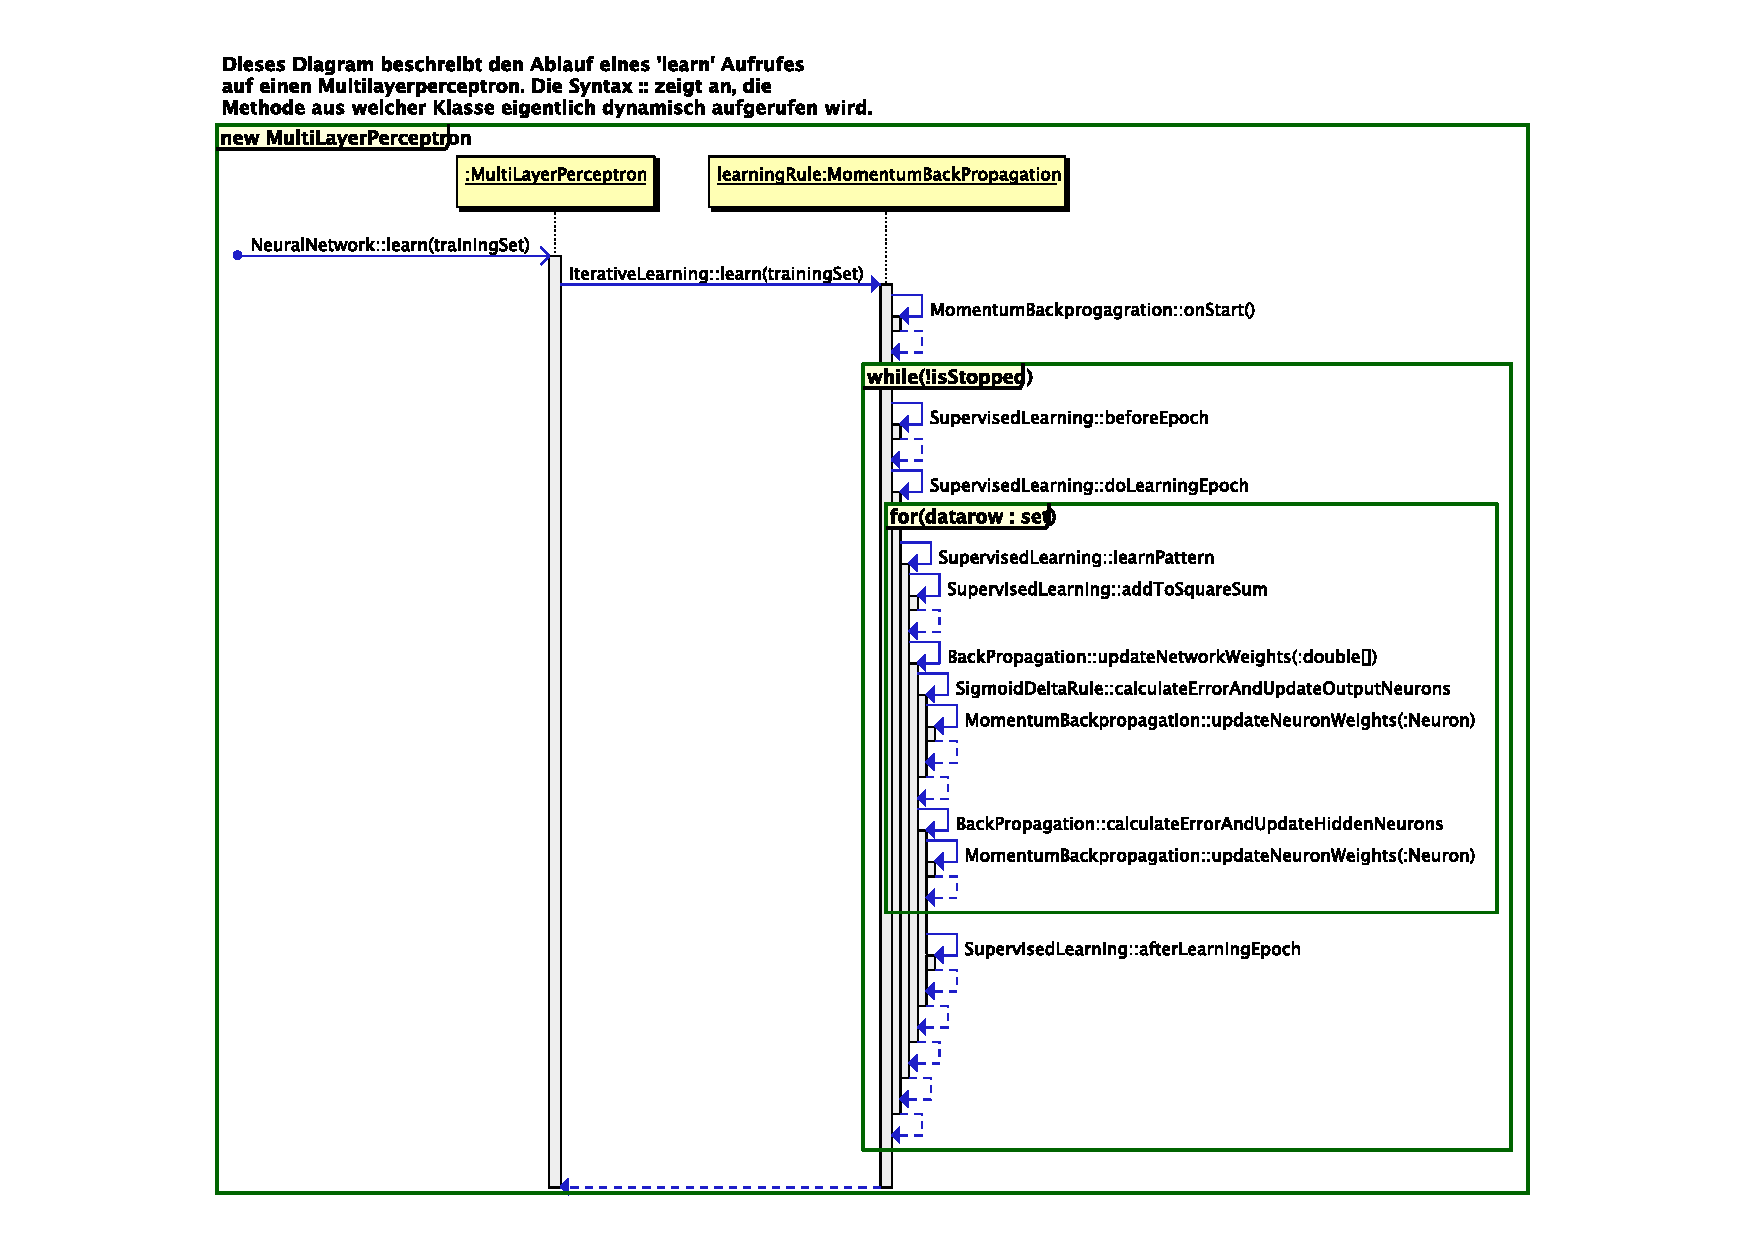
\includegraphics[scale=0.4]{images/Learn.pdf} 
			\end{center}
	\end {frame}			
	
	\begin{frame}[c]\frametitle{Parallelisierungsansätze}
		\begin{itemize}
			\item Layer-Partitionierung
			\item Batch Learning Parallelisierung
			\item Clonebased Parallelisierung
		\end{itemize}	
	\end{frame}
	
	\begin{frame}[c, fragile, allowframebreaks]\frametitle{Layer-Partitionierung}
	    \includegraphics[scale=0.7]{Grafiken/Feingranular.pdf}
	
	\framebreak

		\begin{block}{Layer::calculate()}
			\begin{lstlisting}
			for (Neuron n : this.neurons) 
			    n.calculate();
	 		\end{lstlisting}
 		\end{block}

		\begin{block}{ParallelLayer::calculate()}
	 		\begin{lstlisting}
			ExecutorService service = getExecutor();
			Queue<Future<?>> futures = new LinkedList<>();

			for (NeuronJob j : jobs)
			    futures.add(service.submit(j));
			
			waitForAll(futures);
	 		\end{lstlisting}
	 	\end{block}

 		\framebreak
	
		\begin{itemize}
			\item Erster naiver Ansatz $\rightarrow$ gescheitert!		
			\item Neuer Netzwerktyp: Paralleles neurales Netzwerk
			\item Zu feingranular, Concurrency-Overhead überwiegt erhoffte Zeitersparnis
			% TODO Zahlen hier einfügen
			
		\end{itemize}	
		\begin{center}
			\includegraphics[scale=0.25]{Grafiken/Feingranular.pdf}
		\end{center}
	\end{frame}

	\begin{frame}[c]\frametitle{Exkurs: Batch lernen}
		\begin{center}
			\includegraphics[scale=0.6]{Grafiken/Batchlearning.pdf}		    
		\end{center}	
	\end{frame}

	\begin{frame}[c,allowframebreaks]\frametitle{Batch Learning Parallelisierung}

		\includegraphics[scale=0.58]{Grafiken/Batchparallel_uml.pdf}
		\\
		\textbf{\textit{Paralleles Lernen statt parallelem Netzwerk}}
	\framebreak

		\begin{itemize}
			\item Paralleler Lernvorgang (Netzwerk sequentiell)
			\item Vorteil:
			\begin{itemize}
				\item Saubere, konsistente Schnittstelle
				\item Zugriff auf \textit{protected} Funktionalität
			\end{itemize}
			\item Nachteil: 
			\begin{itemize}
				\item Lernalgorithmus fest 
				\begin{itemize}
					\item Backpropagation
				\end{itemize}
				\item Softwaretechnisch schwierig
				\begin{itemize}
					\item Beispiel: Override mit leerem Body
				\end{itemize}
			\end{itemize}
		\end{itemize}

	\framebreak
		\begin{center}
			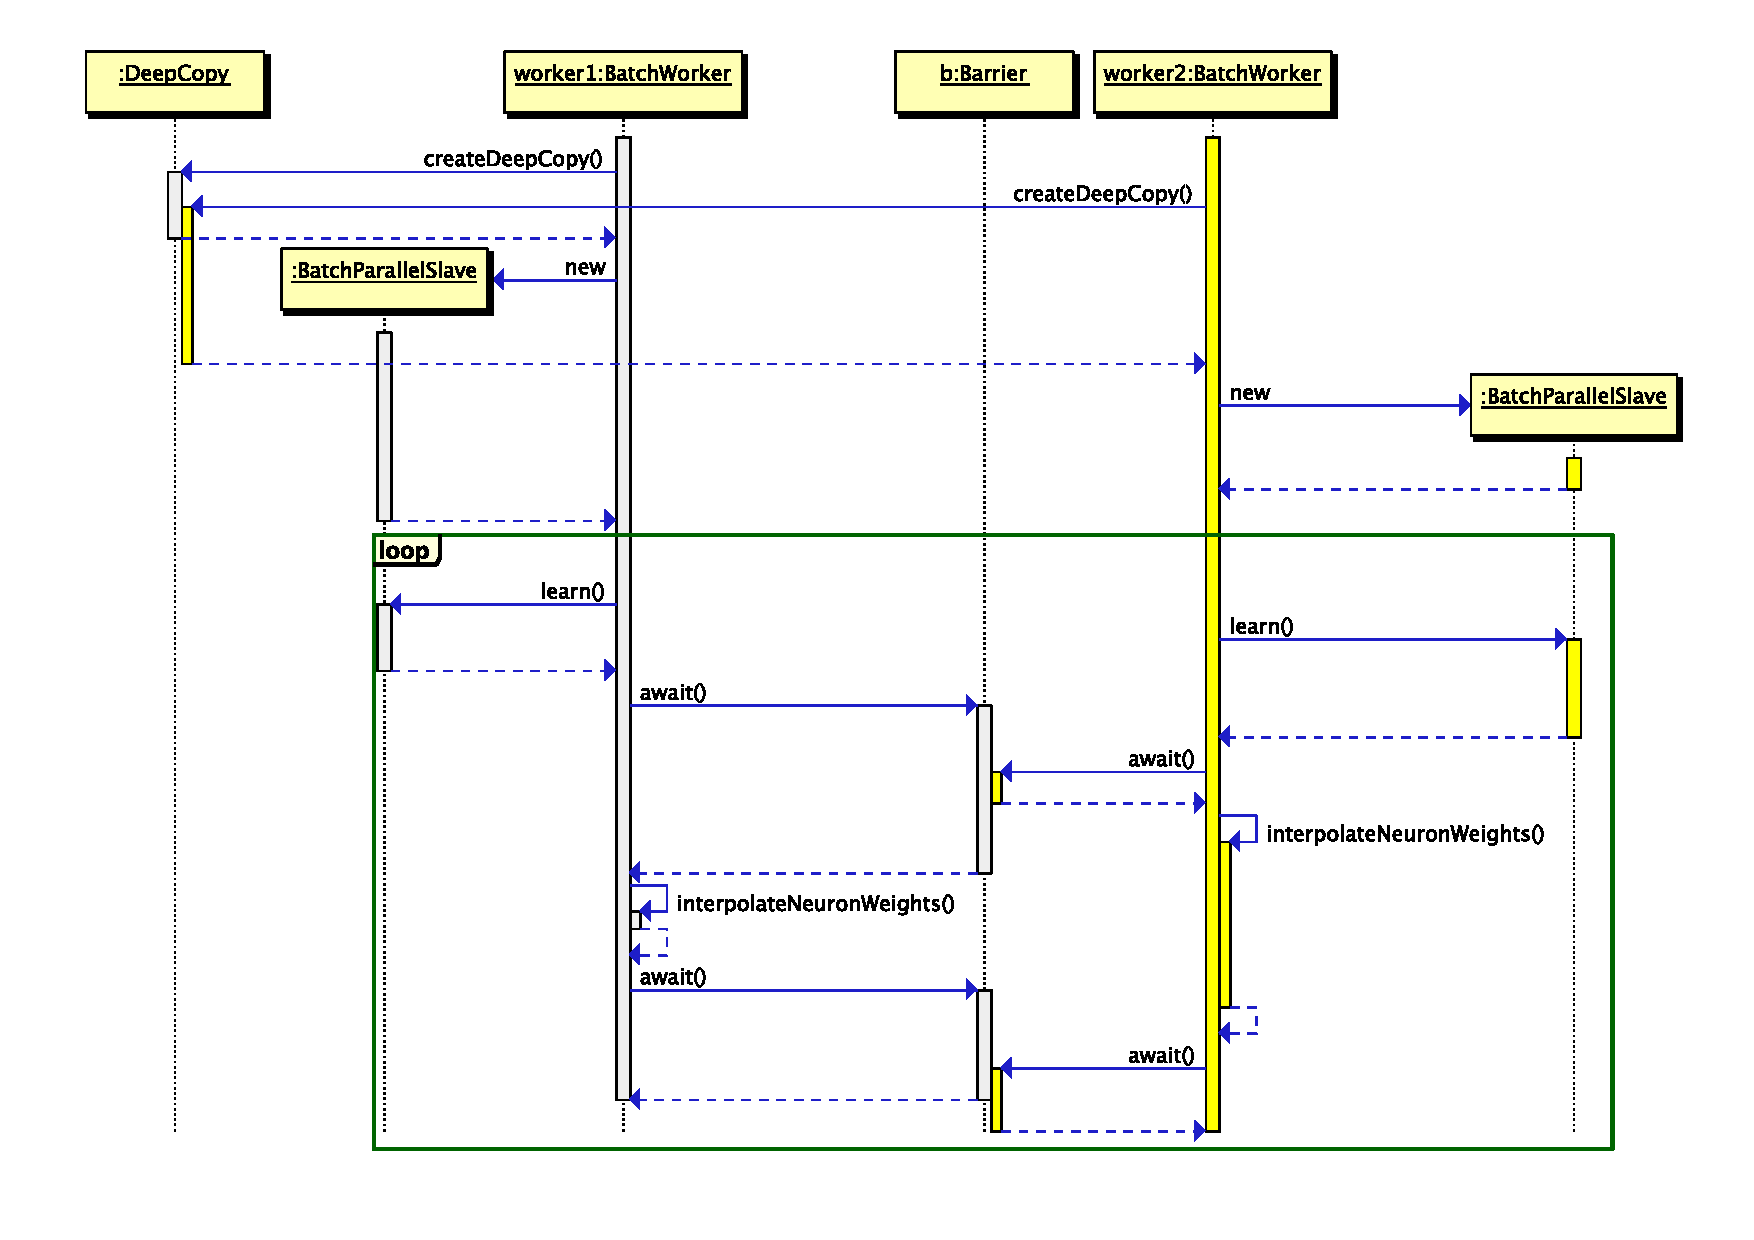
\includegraphics[scale=0.33]{Grafiken/Batch_seq.pdf}
		\end{center}

	\framebreak

		\begin{itemize}
			\item Trainingsdaten auf Worker verteilt
			\item Gewichte interpolieren
			\begin{itemize}
				\item Jeder Thread interpoliert Subset
				\item Dadurch keine Abhängigkeiten
			\end{itemize}
		\end{itemize}
	\end{frame}
	
	\begin{frame}\frametitle{Clonebased Parallelisierung}
		\begin{center}
			\includegraphics[width=.65\textwidth]{images/Parallelisierungsansatz.pdf} 
		\end{center}
	\end{frame}
	
	\begin{frame}\frametitle{Clonebased Parallelisierung}
		\begin{itemize}
			\item ANN wird nach der Erzeugung \glqq geklont\grqq
			\item Ein Klon pro Thread
			\item Unterschiedliche Interpolationsfunktionen
			\item Weitere Parameter
			\begin{itemize}
				\item Synchronisationsintervall
				\item Maximale Anzahl von Iterationen
			\end{itemize}				
			\item Andere Ergebnisgewichte als bei sequentiellem Lernen
			\item Wrapper für ein neuronales Netz
		\end{itemize}
	\end{frame}


	%  TODO: Dominik Clone worker parallelisierung...

	\begin{frame}[c]\frametitle{Technischer Vergleich der Strategien}	
		\begin{tabular}{l|c|c|c|}

		Kategorie &Layerpartitionierung & Batch & Clonebased \\
		\hline
		Was ist parallel? & Netzwerk & Lernen & Lernen\\
		Selbes Ergebnis? & ja & ja (batch) & nein \\

		%TODO fortsetzen
		\end{tabular}
	
	\end{frame}

%TODO: Evaluierung, Zwischenstand, Erwähnen, dass Güte über Zeit und Fehler gemessen wird. Exakt gleich Ergebnis ist nicht erforderlich. Evaluierungsframework

	\begin{frame}[c]\frametitle{Testdaten}
		\begin{block}{Erste Versuche}
		    \begin{itemize}
		    	\item StockExchange - Börsenvorhersage
		    	\item IrisScan Datensatz
		    \end{itemize}
		\end{block}
		\begin{block}{Teilchenkollision (Cern)}
		    \begin{itemize}
		    	\item 15k Datensätze
		    	\item Eingabe: 2853 Sensorwerte
				\item Ausgabe: Ist das Ereignis interessant oder nicht? 
				%Schwarzes Loch oder nicht?
		    \end{itemize}
		\end{block}		
	\end{frame}

	\begin{frame}\frametitle{Evaluationsframework}
		\begin{block}{Score}
			wird bestimmt durch
		    \begin{itemize}
		    	\item Fehler (auf Testdaten)
		    	\item Laufzeit
		    \end{itemize}
		\end{block}
		\begin{block}{Vorgehen}
		    \begin{enumerate}
		    	\item Permutation der Daten
		    	\item Aufteilung in Trainings- und Testdaten
				\item $foreach$ ILearner L $do$
				\begin{itemize}
					\item Lerne Trainingsdaten und messe Ausführungszeiten
					\item Berechne Fehler auf Testdaten
				\end{itemize}
				\item Wiederhole ab 1 bis gewünschte Anzahl an Läufen erreicht
		    \end{enumerate}
		\end{block}
	\end{frame}
	
	\begin{frame}\frametitle{Aktuelle Evaluationswerte}
		\begin{block}{Experiment-Konfiguration}
			\begin{itemize}
				\item 5000 Datenreihen aus CERN-Satz, 1:1 Trainings-/Testdaten
				\item Intel Core2Quad Q6600, 4 Kerne à 2,4GHz, 8GB RAM
				\item JDK 7
			\end{itemize}
		\end{block}
		\includegraphics[width=0.51\textwidth]{images/eval_speedup.png}
		\includegraphics[width=0.49\textwidth]{images/eval_error.png}
	\end{frame}

\end{document}

